\chapter{Android Lint}
\label{android_lint}
\section{Visão geral}

Android Lint é uma ferramenta oficial disponibilizada pela Google no Android 
Development Toolkit que analisa o código-fonte de projetos Android em busca de 
potenciais erros. Está disponível tanto como uma ferramenta de linha de comando, 
quanto integrado com IDEs, como o Android Studio. Exemplos de erros analisados incluem:

\begin{itemize}
  \item{Traduções incompletas (e traduções não utilizadas)}
  \item{Problemas de performance de layout}
  \item{Recursos (arquivos de imagens e sons, por exemplo) não-utilizados}
  \item{Problemas de internacionalização e acessibilidade}
  \item{Problemas relacionadas a ícones}
  \item{Problemas de usabilidades}
  \item{Erros no arquivo de manifesto, um elemento central no mecanismo de variabilidade
  da plataforma Android \cite{mechanisms}}
\end{itemize}

Atualmente, o Android Lint possui cerca de 190 regras, que agrupam os erros em 
diversos graus de severidade e categorias. Os graus de severidade são 5, que vão 
de apenas informativos, onde não necessariamente é um erro mas que algo no código 
deve ser analisado, até fatal, em que existe um erro crítico no projeto, a ponto 
de falhar a criação do arquivo APK. Quanto às categorias podemos encontrar segurança, 
acessibilidade, internacionalização, usabilidade entre outras. Analisando essa 190 
regras previamente definidas, podemos relacionar cerca de 70 com algum tipo de 
variabilidade ou padrão definido pela plataforma. Como exemplo, podemos citar as 
regras "ButtonOrder", que verifica se a ordem dos botões na interface estão de 
acordo com o padrão de design sugerido pela documentação oficial e "NewApi", 
relacionado a variabilidade de versões da API, que aponta chamadas de métodos 
não-disponíveis em todas as versões da API para qual a aplicação foi desenvolvimento 
(de acordo com a versão mínima específica no arquivo de manifesto). O apêndice 
\ref{apd_cheks_uteis} apresenta uma lista completa dessas regras. 

Para que o Android Lint aplique a analise de uma regra é necessário definir quais 
regras deverão ser utilizadas, o que pode ser feito no arquivo {\it build.gradle} do 
projeto na seção {\it lintoptions}, conforme mostra figura \ref{lintoptions}:

\begin{figure}[h]
    \centering
    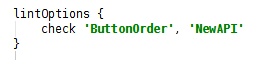
\includegraphics[width=5cm]{img/lintoptions.png}
    \caption{Trecho do arquivo build.gladle, indicando que as regras ButtonOrder e 
    NewApi devem ser executadas}
    \label{lintoptions}
\end{figure}

\section{Criação de novas regras}

Quando são necessárias regras não definidas pelo Lint, novas regras podem ser criadas. 
No entanto, devemos observar que a API do Lint ainda não está estável. Assim, mudanças 
deverão ser necessárias no futuro. Além disso, não existe uma documentação adequada 
dessa API, sendo necessária a leitura do código-fonte tanto da API quanto das regras 
pré-definidas.

Para criar uma nova regra, precisamos fazer a distinção entre “issue” e “detector”. 
“Issue” é um tipo de problema que iremos localizar e mostrar para o desenvolvedor. 
O responsável por fazer essa busca e detecção é um “Detector”.

O tipo de artefato do projeto relacionado ao Issue e que será analisado pelo 
Detector é denominado escopo, que pode ser: arquivos de recursos, código-fonte Java, 
arquivos .class, arquivos de configuração do Proguard e arquivo de manifesto. Quando 
um Issue é criado, seu escopo é definido a partir da classe “Scope”. Por exemplo, 
um Issue relacionado a problemas no arquivo de manifesto tem seu escopo definido 
com Scope.MANIFEST. Esse escopo também terá impacto em quais interfaces um detector 
deverá implementar.

De acordo com a análise necessária, detectors deverão implementar uma ou mais das 
seguintes interfaces: Detector.XmlScanner, Detector.JavaScanner, Detector.ClassScanner. 
Por exemplo, para um detector com escopo para o arquivo de manifesto, deverá implementar 
a interface XmlScanner. E então deveremos implementar o método “visitDocument”, que será 
chamado uma vez para cada arquivo XML, e irá retorno o DOM do XML, que poderá ser utilizado 
para a análise necessária. Contudo, muitas vezes estamos interessados em um tag ou um atributo 
em particular, ou em um conjunto deles. Nesses casos, podemos implementar os métodos 
“getApplicableElements” e/ou “getApplicableAttributes”, que retornam uma lista de strings 
com os nomes das tags ou atributos. Então, implementamos os métodos “visitElement” e/ou 
“visitAttribute”, que serão chamados para cada item das listas retornadas pelos métodos 
citados anteriormente.

Para analisar código-fonte Java, deve-se implementar a interface JavaScanner, da 
qual alguns métodos deverão ser implementados. Entre eles o “createJavaVisitor”, 
que deverá retornar um objeto AstVisitor do projeto Lombok\footnote{https://projectlombok.org/}, 
utilizado pelo Lint para representar ASTs. Também existem alguns métodos para facilitar 
a analise, como o “getApplicableNodeTypes” que especifica tipos de nós a serem analisados 
e “getApplicableMethods”, onde pode ser definido um conjunto de métodos da aplicação
em que estamos interessados.

Já para analise de bytecode a interface ClassScanner é que deverá ser implementada. 
Lint usa a biblioteca ASM\footnote{http://asm.ow2.org/} para processar arquivos .class, que percorre os arquivos 
e produz um objeto ClassNode, que é então passado para cada ClassScanner. Os detectors 
poderão usar esses ClassNodes para analisar o bytecode conforme a necessidade.

\subsection{Reportando erros}
O Lint fornece uma infraestrutura simplificada para reportar os problemas encontrados. 
Basta chamar o método report() no objeto context (que é passado para cada método do detector.). 
Além do problema (Issue) em si, também pode ser fornecido uma localização, um “escopo do nó”, 
e uma mensagem. A localização é o ponto onde o erro ocorreu, o local no DOM se for um XML ou 
o nó da árvore AST se for um código-fonte Java, que irá permitir saber o local exato do arquivo 
onde ocorreu o erro. O “escopo do nó” é o nó AST/XML mais próximo em volta do local do erro. 
Usualmente é o mesmo nó de onde foi criado a localização.

